\section{Treatment of the singularity}
\label{sec:innerCenter}
The cylindrical coordinate system has a singularity at the axis (where $\rho=0$).
In other words, functions are not well defined in this point, and hence it is a bad idea to have a grid point there.
One way to avoid this problem is to put the grid points close to, but not at the very axis.
At the same time, as mentioned in \cref{sec:BCInnerRho}, there is a need of artificial boundary conditions as the domain covers $\rho \in \;]0, L_\rho[$.

\subsection{Ghost point for the radial derivative}
\label{sec:ghostRhoDeriv}
We immediatley observe that having a boundary condition at the singularity is a bad idea due to the singularity.
It is also a bad idea to use one sided FD schemes around this point, as this will prevent communication of information through the axis.

One way to circumvent the problem is to put the innermost point in rho $\Delta \rho$ appart from each other, where $\Delta \rho$ is the grid spacing.
I. e. the innermost points are both located $\frac{\Delta \rho}{2}$ from the axis, diametrically opposite of each other, as depicted on \cref{fig:innerRho}.
%
\begin{figure}[htb]
    \centering
    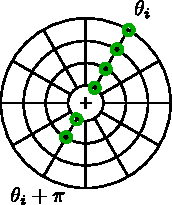
\includegraphics[width=0.5\textwidth]{fig/innerGhost}
    \caption{\textit{
The solid lines black lines represent the coordinate curves of a mesh with $4$ points in the $\rho$ direction (excluding the outermost ghost point depicted with a dashed black line), and $8$ points in the $\theta$-direction.
The green solid circles represents the inner grid points at $\theta=\theta_i$, with the corresponding ghost points at $\theta=\theta_i + \pi$ depicted in green dashed circles.
    }}
    \label{fig:innerRho}
\end{figure}
%
In this solution, the ghost points for the innermost grid points in $\rho$ (those closest to the singularity) will be set to the value of the innermost grid point which lies $\theta + \pi$ away.
The next ghost point will be set to the value of the second innermost internal point which lies $\theta + \pi$ away, and so on.
In this thesis, only one ghost point is used.
With this method the second order FD stencil for the radial derivative becomes
%
\begin{align*}
    \L.\parti{f}{\rho}\R|_{\rho=\frac{\Delta \rho}{2}} \simeq
    \frac{-f\L(-\frac{\Delta \rho}{2}, \theta\R) + f\L(\frac{3\Delta \rho}{2}, \theta\R)}{2\Delta \rho}
    =
    \frac{-f\L(\frac{\Delta \rho}{2}, \theta+\pi\R) + f\L(\frac{3\Delta \rho}{2}, \theta\R)}{2\Delta \rho}
\end{align*}
%
for the innermost point.
This method was used in \cite{Naulin2008}, and is second order convergent for a second order stencil as shown in \cref{sec:MES}.

\subsection{The inner boundary condition for \texorpdfstring{$\phi$}{the potential}}
\label{sec:innerPhiBC}
%
We also need an artificial ghost point for the innermost point in $\rho$ for inversion method described in \cref{app:lapInv}.
As the inversion in the $\rho$ direction will be done for each mode, the method described in \cref{sec:ghostRhoDeriv} is not directly applicable.

A method to do this, is to set the inner ghost point depending on the evenness of the mode.

If the mode is even, the mode under consideration would have the same value diametrically opposite of the innermost point.
Notice that this is true for every point sitting on the same radius.
Hence, the ghost point for the inner $\rho$ value is set to the same as the value at the innermost $\rho$.

If the mode is odd, the mode under consideration would have value of the point diametrically opposite of the innermost point, but with a changed sign.
Thus, the ghost point for the inner $\rho$ value is set to the negative of the value at the innermost $\rho$.
This is depicted in \cref{fig:BCLaplace}, and was first used in
%
\begin{figure}[h!]
    \centering
    \begin{subfigure}[t]{0.5\textwidth}
        \centering
        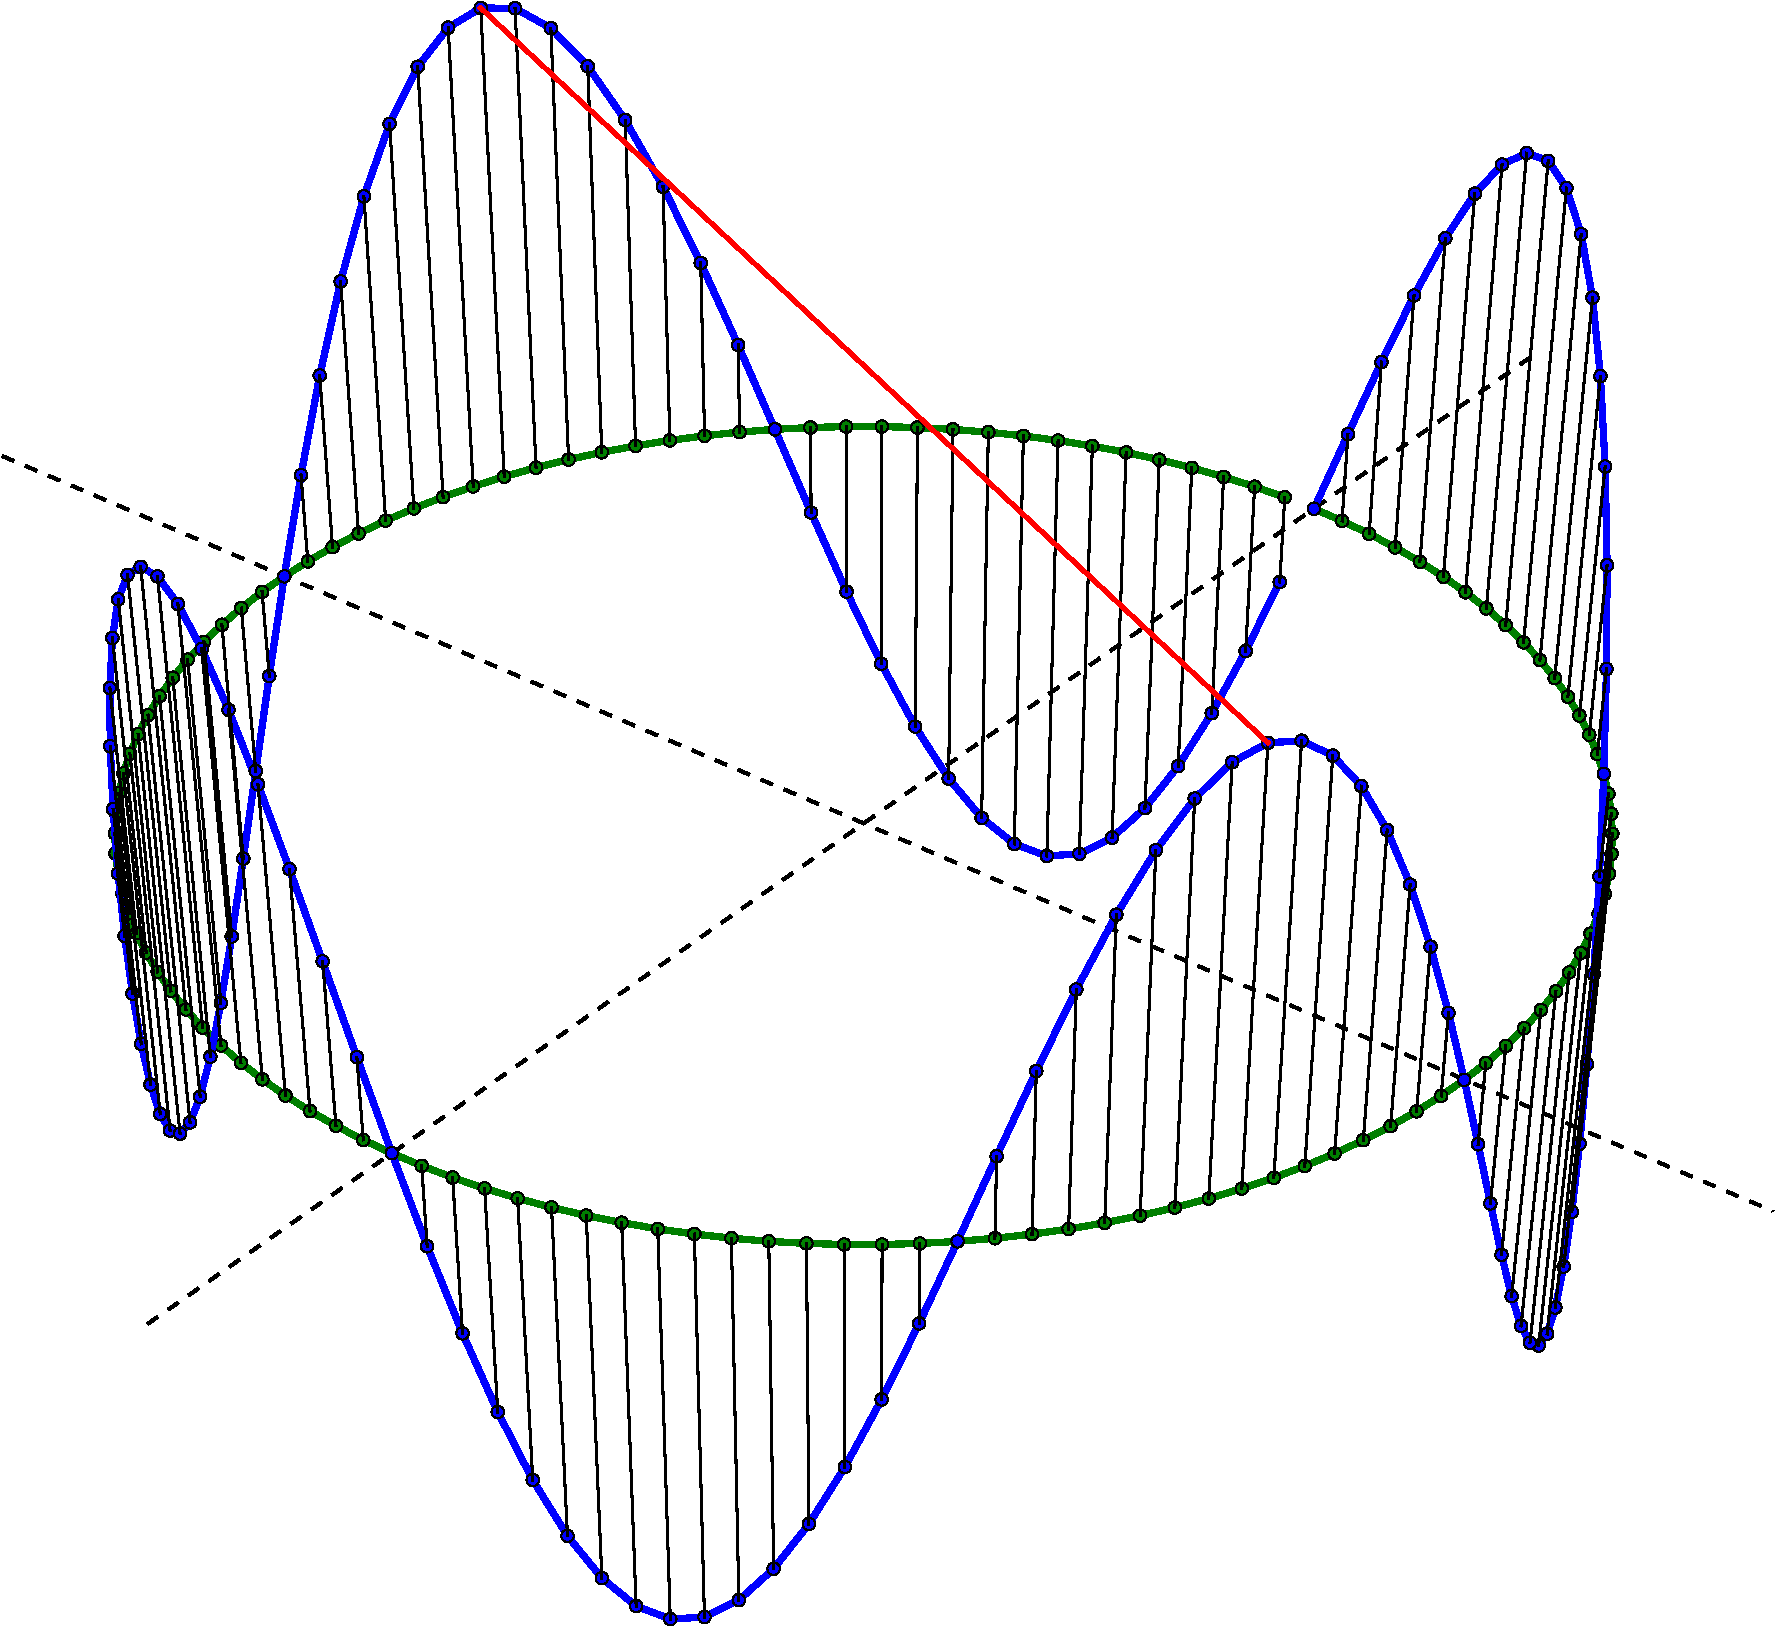
\includegraphics[width=0.8\textwidth]{fig/mode_4}
        \caption{An even mode.}
    \end{subfigure}%
    \hfill
    \begin{subfigure}[t]{0.5\textwidth}
        \centering
        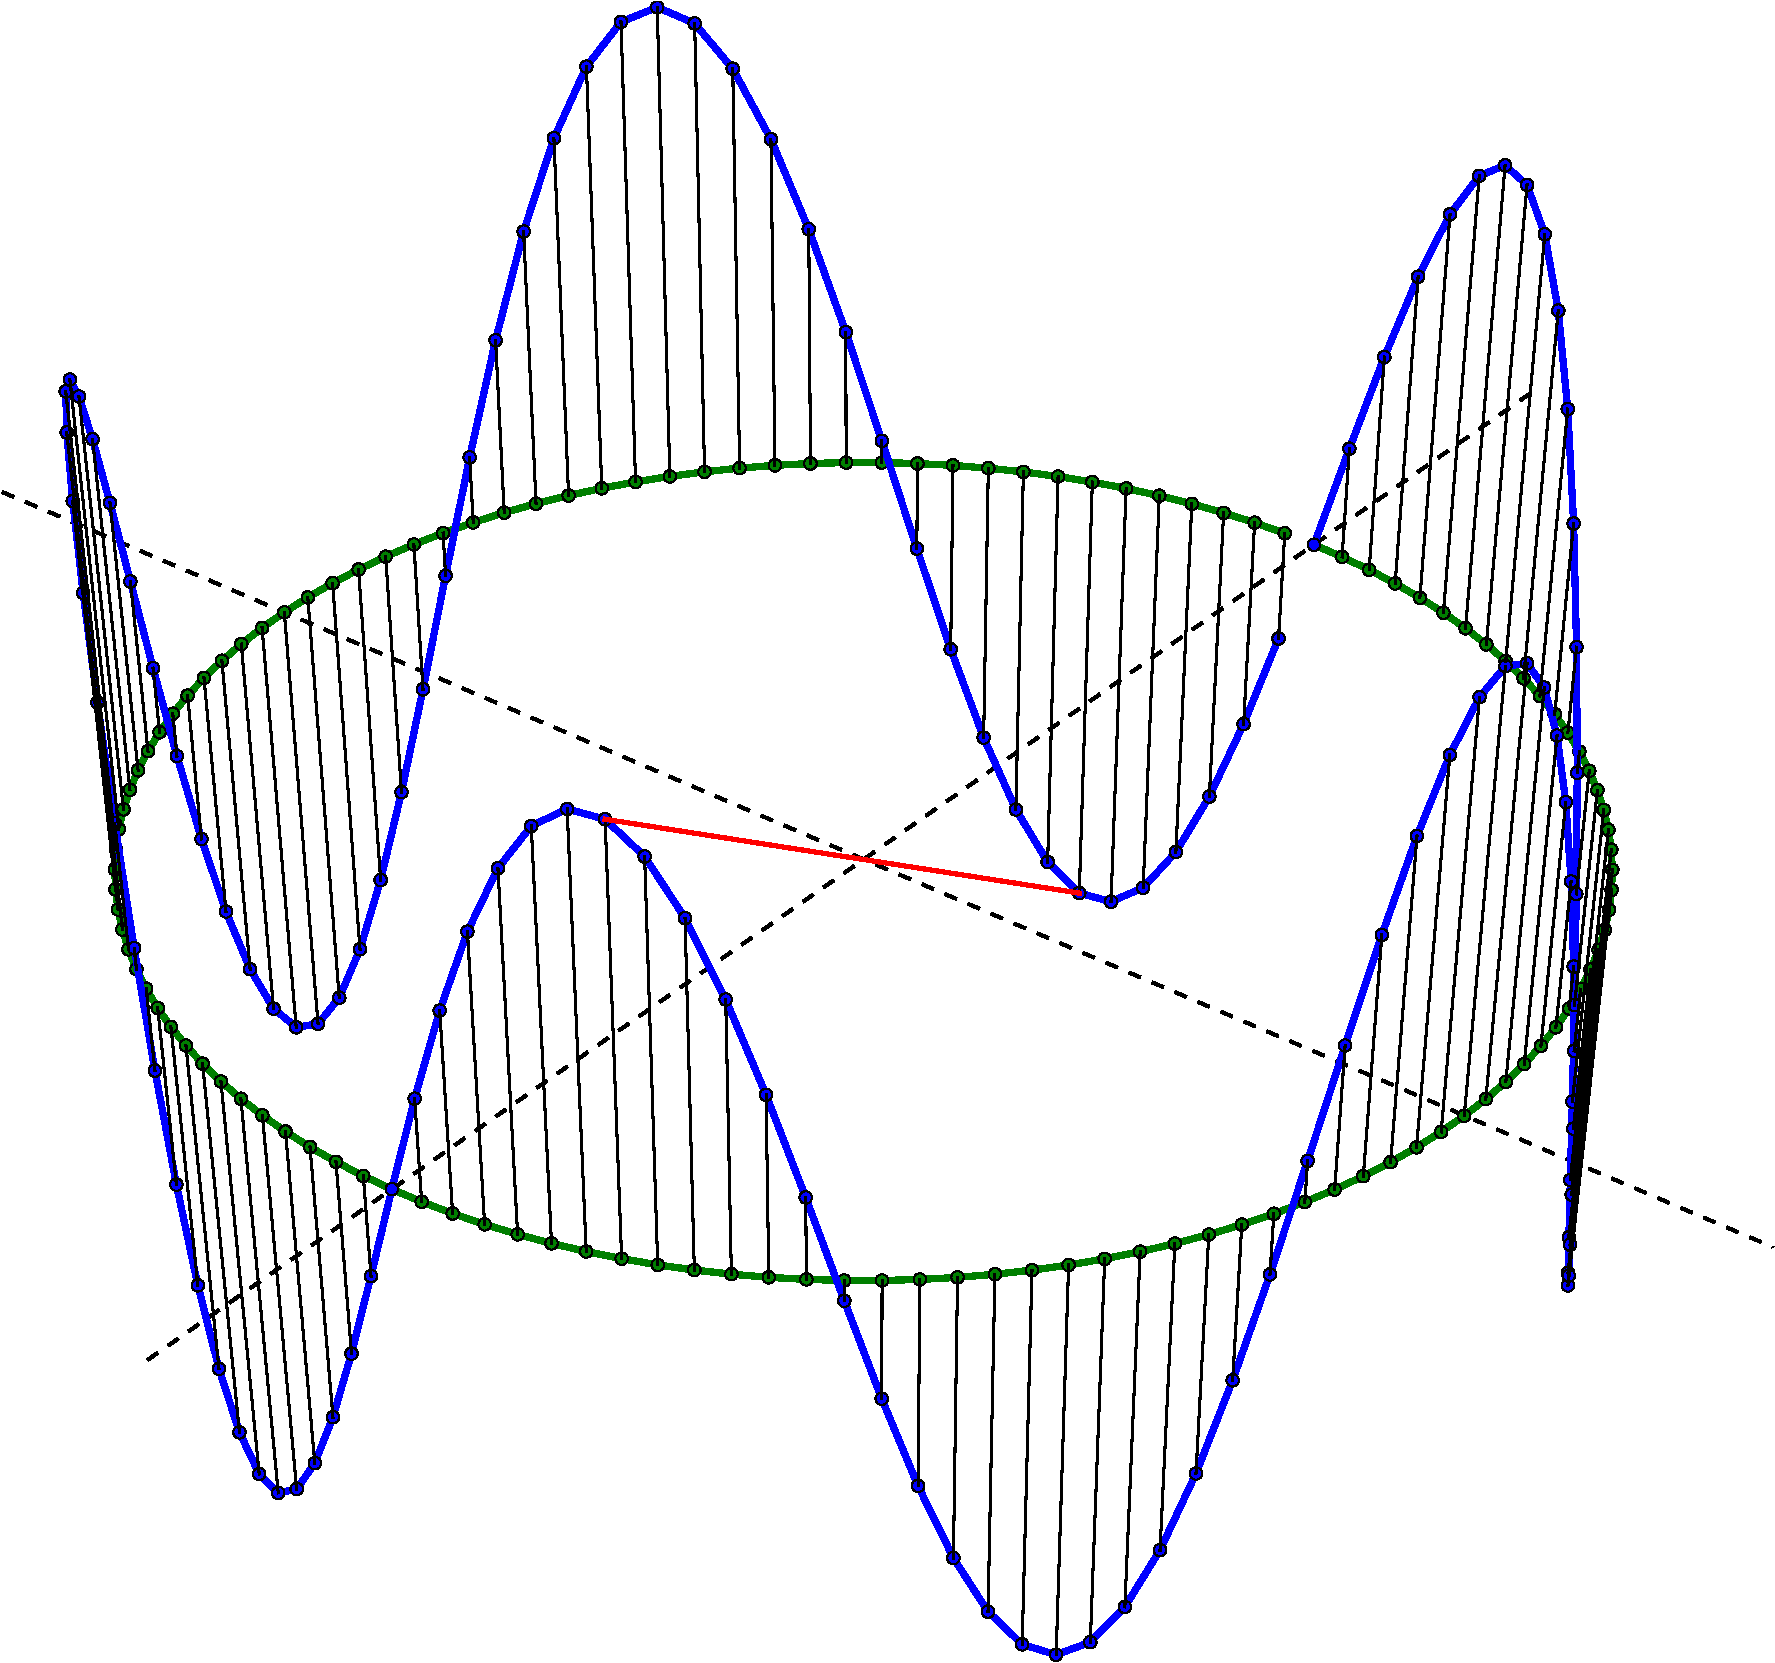
\includegraphics[width=0.8\textwidth]{fig/mode_5}
        \caption{An odd mode.}
    \end{subfigure}
        \caption{The point diametrically opposite for a mode located at radius $\rho$ has the same value as the point under consideration for an even mode, but the same value with a changed sign for even modes.
        The red soid line connects points diametrically opposite of each other.}
    \label{fig:BCLaplace}
\end{figure}
